\documentclass{beamer}
\usepackage{graphicx}
\usepackage[spanish]{babel}
\usepackage[utf8]{inputenc}
\setbeamertemplate{navigation symbols}{}
\usepackage{beamerthemeshadow}
\begin{document}
\title{Aplicaciones Web Desconectadas}
\author{Defossé Nahuel, van Haaster Diego Marcos}
\date{15 de Diciembre de 2009}

\begin{frame}
\titlepage
\end{frame}

% \frame{
%     \frametitle{Contenido de la presetnación}
%     \tableofcontents
% }

\section{Introducción}
\subsection{Contexto}

\begin{frame}
    \frametitle{¿Qué es Web?}
    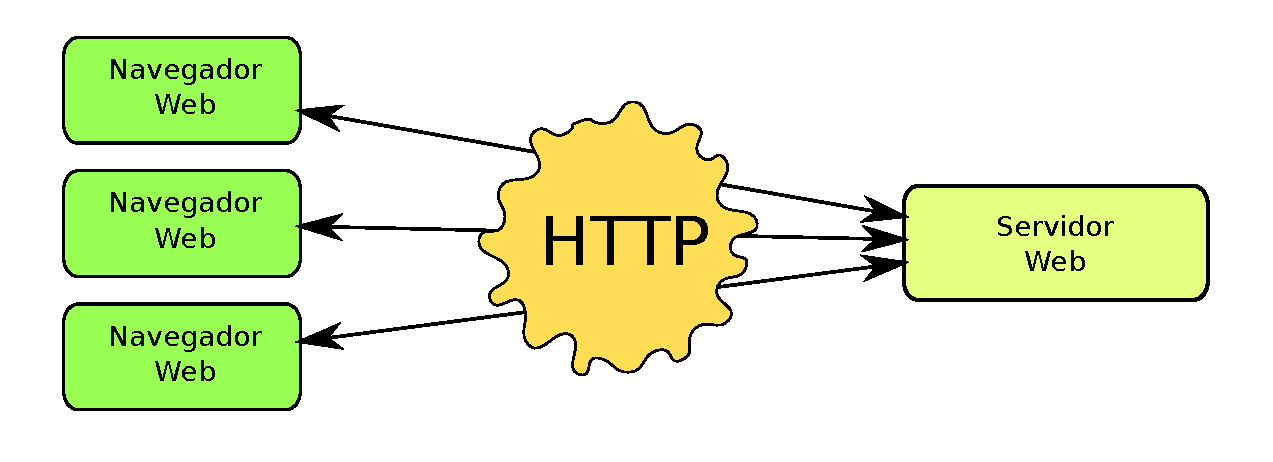
\includegraphics[scale=0.5]{intro.pdf}
\end{frame}
    

\begin{frame}
    \frametitle{¿Qué es una aplicación Web?}
    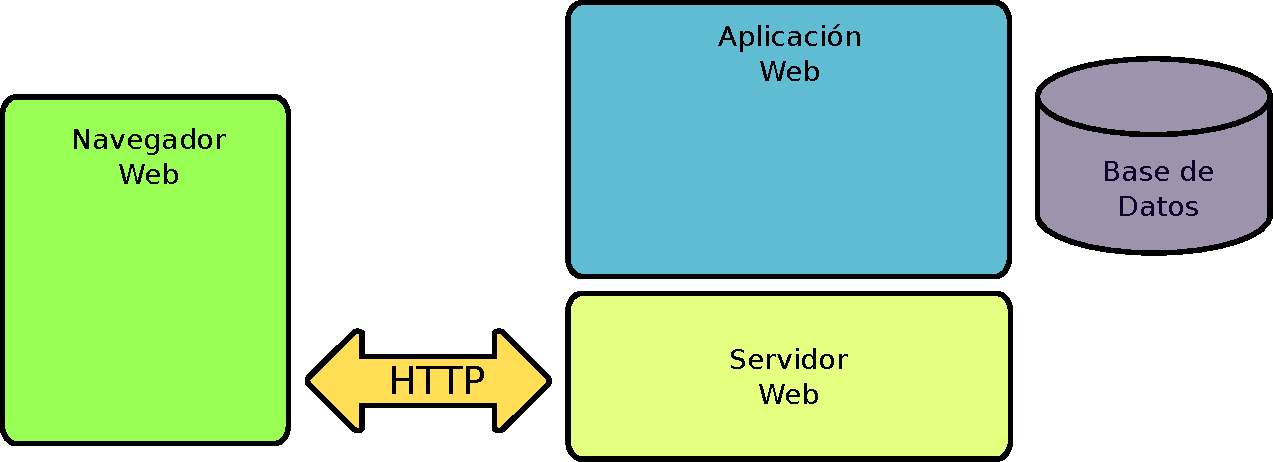
\includegraphics[scale=0.5]{general.pdf}
\end{frame}

\begin{frame}
    \frametitle{¿Qué es una aplicación Web Hoy?}
    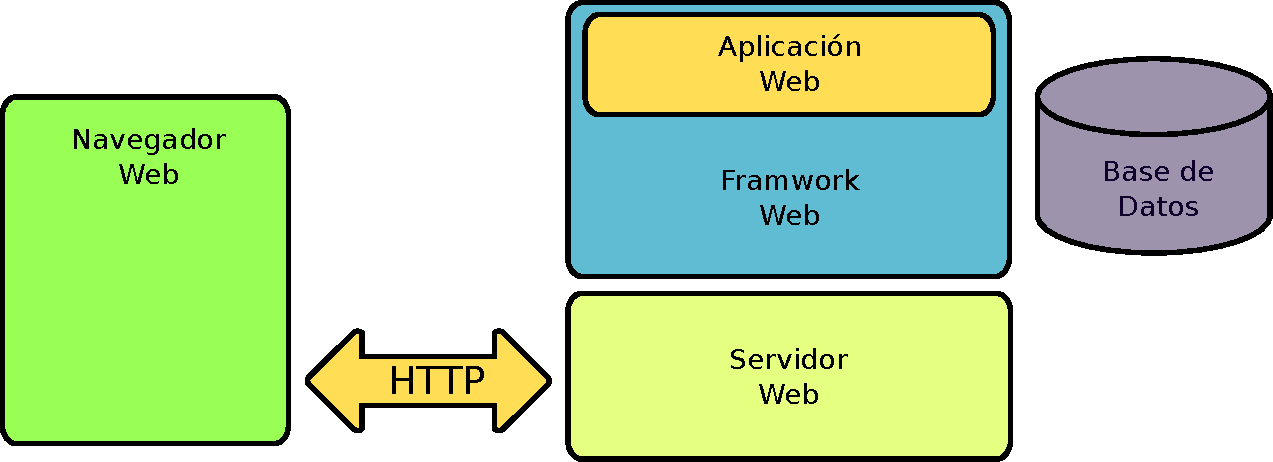
\includegraphics[scale=0.5]{general_con_fw.pdf}
\end{frame}

\subsection{Objetivos}
\frame{
    \frametitle{Objetivos Principales}
    \begin{block}{Objetivo Principal}
    
    ``Extender un framework de aplicaciones web existente, {\bf Open Source},
              de manera que una aplicación realizada sobre éste pueda ser ejecutada
              en el cliente de manera desconectada con un mínimo de modificaciones.
              Para permitir que la aplicación pueda ejecutarse en el cliente, se
              implementará''
        \begin{itemize}
        \item Persistencia del modelo de datos en el cliente.
        \item Subconjunto de acciones disponibles en modo desconectado
        \item Primitivas de sincronización entre la aplicación del cliente y la aplicación web que le dio origen
        \end{itemize}
    \end{block}

}


\frame{
    \frametitle{Objetivos Secundarios}
    \begin{itemize}
        \item{{\bf Open Source}\\
                Coste de licenciemiento nulo y aseguramiento de la continuidad
        }
        \item{{\bf Multiplataforma}\\
            Windows, Linux, Mac y móviles (donde exista un browser)
        }
        \item{{\bf Adaptación mínima de aplicaciones existentes}\\
            Integración con un Frameworks Web \par
            Reutilizar los conceptos/patrones del framework para una rápida asimilación de los desarrolladores.
        }
    \end{itemize}
}

\subsection{Framework Web}
\begin{frame}
\frametitle{Framework Web - Django}
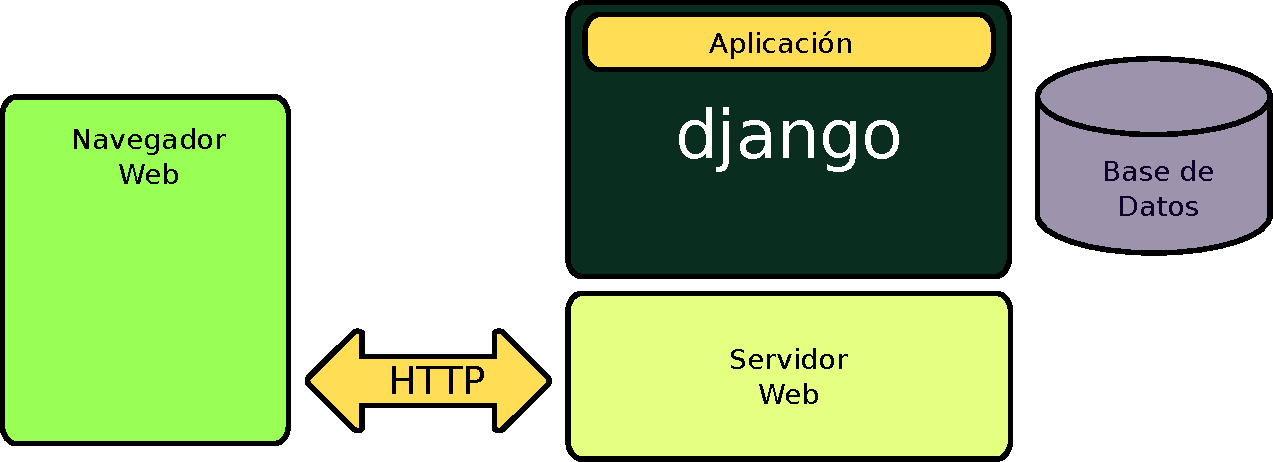
\includegraphics[scale=0.5]{fw_django.pdf}
\end{frame}

\begin{frame}
\frametitle{Framework Web - Django - Componentes}
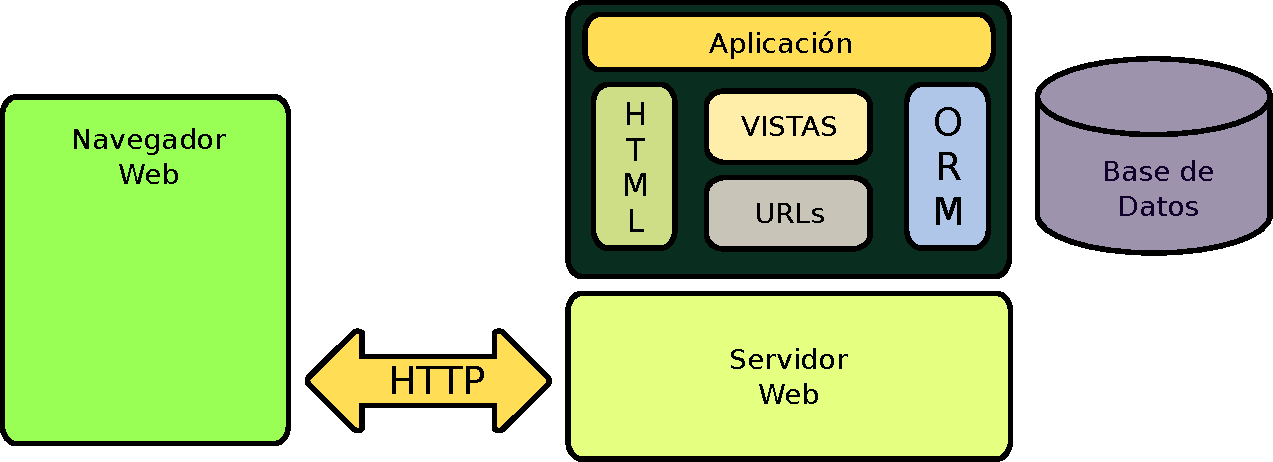
\includegraphics[scale=0.5]{fw_django_comp.pdf}
\end{frame}

\subsection{Principales Obstáculos}
\frame{
    \frametitle{Carencias de los navegadores}
    \itemize{
        \item{\bf Servidor Web}\\
        Sin servidor, el navegador solo posee la {\bf cache}
        \item{\bf Base de Datos} \\
        Un navegador no posee un mecanismo de almacenamiento
        \item{\bf Lenguaje de Programación Consistente}\\
        Cada navegador implementa a su manera {\bf JavaScript} y {\bf DOM}
        \item{\bf Concurrencia} \\
        Los eventos son atendidos en el bucle principal
        \item{{\bf Conectividad con el entorno del cliente}\par
            Escritorio $\not=$ Espacio de URLs
        }
    }
}

%\subsection{Tecnologías Existentes}
\frame{
     \frametitle{Principales alternativas}
     
     
     \begin{columns}[c]
     \begin{column}{5cm}
         \itemize{
             \item {\bf Microsoft Silverlight}\\
             \item {\bf Sun JavaFX}
             \item {\bf Adobe AIR}
             \item {\bf Mozilla XUL}
         }
     \end{column}
     \begin{column}{5cm}
        
\includegraphics[scale=0.2]{microsoft_silverlight_c.jpg}\\
        
\includegraphics[scale=0.3]{javafx_logo_color_1.jpg}\\
        
\includegraphics[scale=0.16]{adobe_air_realin.png}

     \end{column}
     \end{columns}
     

%    \pause
%    \\
%    Esteas tecnologías se alejan de los estándares de la Web.
    % Decir que la web 2.0, desde el punto de vista tecnologico
    % tiende a integrar serivcios en una plataforma estandar abiertos (HTML, JS + libs, etc.)
    % Estos NO.
}

\frame{
    \frametitle{JavaScript}
    \par{Un lenguaje con {\it mala} reputación con:}
    \begin{itemize}
          \item Objetos
          \item Patrones Propios (Closures, Module, etc.)
          \item Muchas librerías                    
    \end{itemize}
    \vfill
    \par{
        
\includegraphics[scale=0.4]{prototype.png}\hfill
        
\includegraphics[scale=0.2]{dojo.png}\hfill  
        
\includegraphics[scale=0.4]{jquery.png}
    }
    \par{
        
\includegraphics[scale=0.2]{yui.jpg}\hfill
        
\includegraphics[scale=0.5]{DHX_logo.jpg}\hfill
        
\includegraphics[scale=0.3]{mootools.png}
        
    
    }
    
}

\frame{
    \frametitle{JavaScript - Según Mozilla}
    
    \begin{columns}[c]
         \begin{column}{5cm}
             \itemize{
                 \item Generadores e Iteradores
                 \item Varias ayudas para una mejor programación OO
                 \item Sabor Pythonico :)
             }
         \end{column}
         \begin{column}{5cm}
            
\includegraphics[scale=1.2]{mozilla.png}
            
    
         \end{column}
     \end{columns}
    
    
        
    

}

\frame{
    \frametitle{Google Gears}
    \par{
        Plugin para los navegadores\hfill
\includegraphics[scale=0.3]{gears.png}
    }
    \itemize{
        \item{\bf Local Server}
        \item{\bf Data Base}
        \item{\bf Worker Pool}
        \item{\bf Desktop}
    }
    
}
\section{Desarrollo}
\subsection{Propuesta}
\frame{
    \frametitle{Gears}
    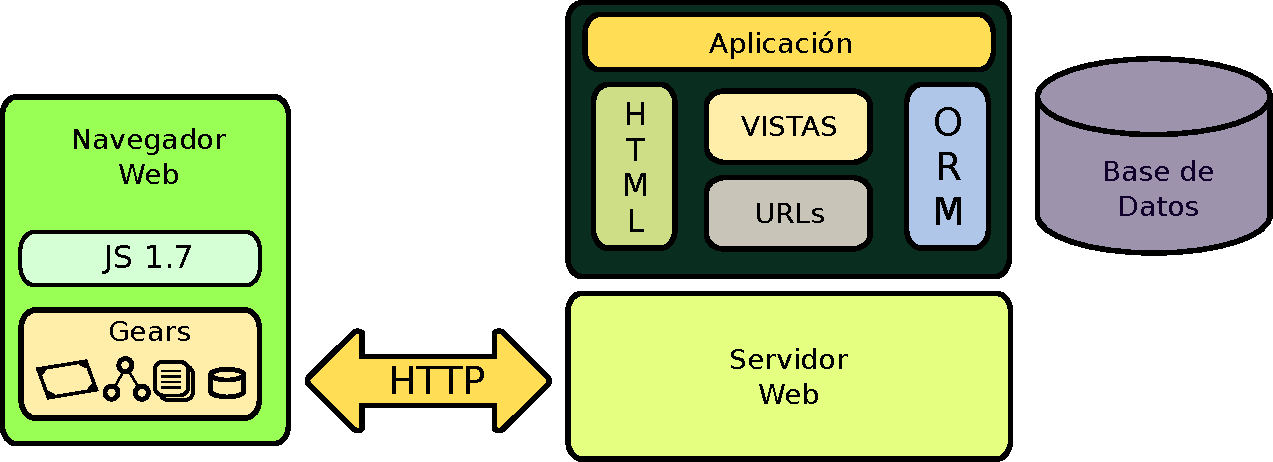
\includegraphics[scale=0.5]{fw_django_comp_gears.pdf}
}

\frame{
    \frametitle{¿Django Desconectado?}
    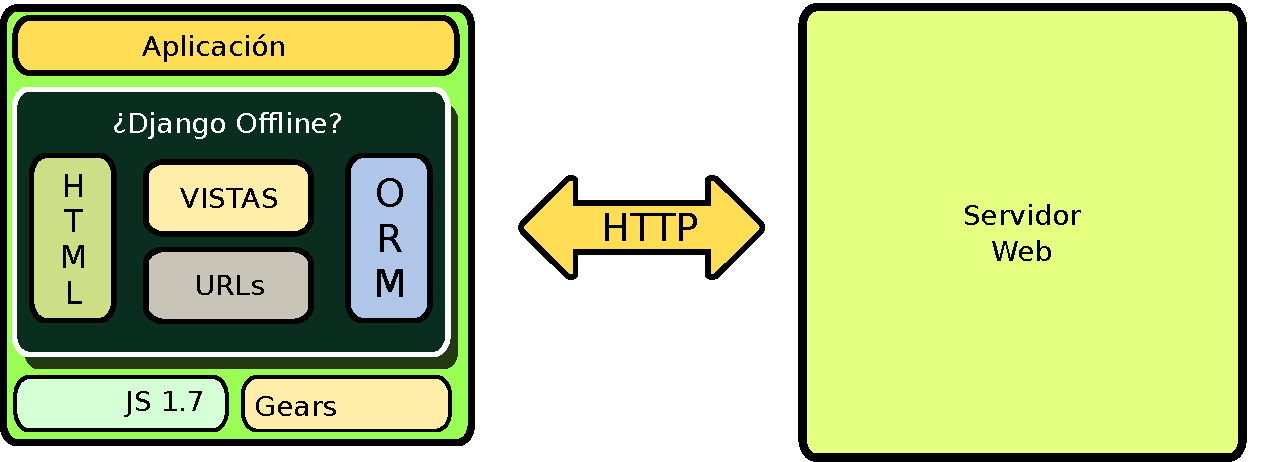
\includegraphics[scale=0.5]{fw_desconectado.pdf}
}

\subsection{Solución}
\frame{
    \frametitle{Doff y Protopy}
    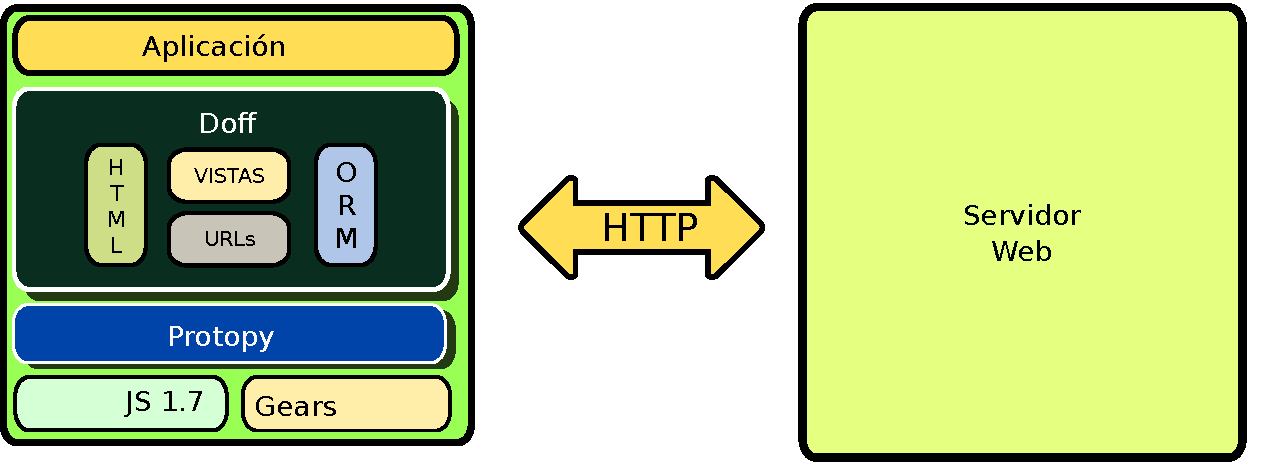
\includegraphics[scale=0.5]{fw_doff_protopy.pdf}
}
\subsubsection{Librería de JavaScript}
\frame{
    \frametitle{Protopy - Librería de JavaScript}
    
            {\bf Objetivos:}\par
                \begin{itemize}
                        \item{Interfase Pythonica para desarrolladores}
                        \item{Promover la reutilización de código}
                        \item{Control de la página y eventos(DOM) - Trabajo cotidiano
                        del desarrollador web de {\it front-ends}}
                        \item{Soporte de el framework desconectado.}
                        \item{Interfase con las tecnologías de persistencia y ejecución
                        offline.} 
                \end{itemize}     
         
    
        
}
\frame{
    \frametitle{Componentes de Protopy}
        \begin{columns}[c]
         \begin{column}{5cm}
    
            \begin{itemize}
                \item {\bf Módulos}
                \item {\bf Clases}
                \item {\bf DOM}
                \item {\bf Eventos}
                \item {\bf AJAX}
             \end{itemize}
         \end{column}
         \begin{column}{5cm}
            
\includegraphics[scale=0.5]{protopy.png}
         \end{column}
     \end{columns}                       
    
    

}

\frame{
    \frametitle{Componentes de Protopy}
    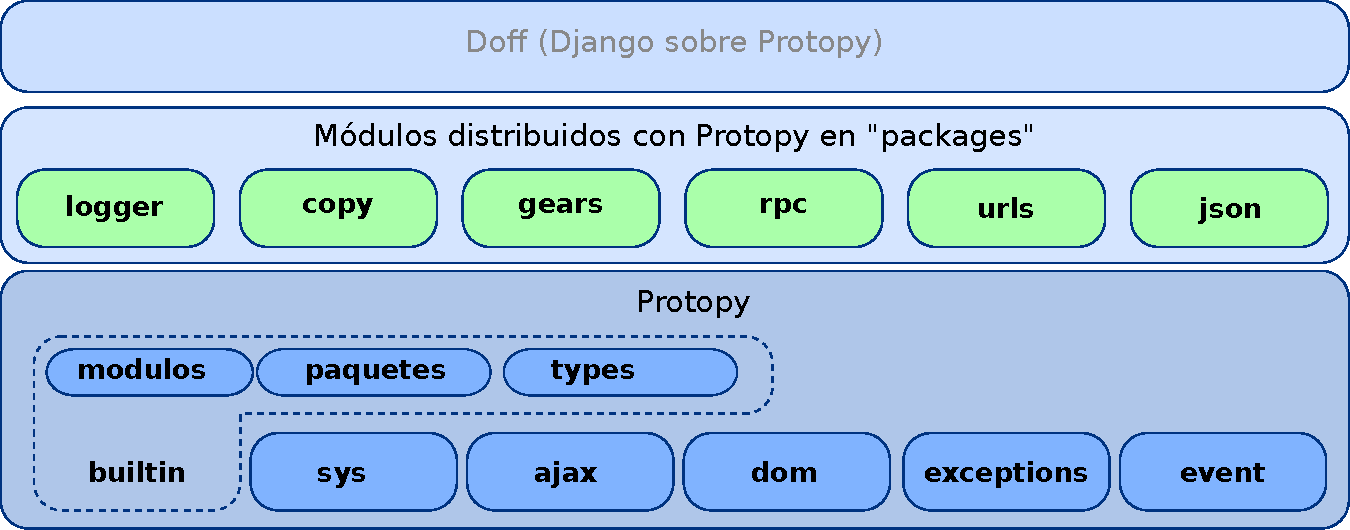
\includegraphics[scale=0.47]{esquema_protopy.pdf}
}

\frame{
    \frametitle{Doff - Objetivos}
    {\bf Objetivos:}
    \itemize{
        \item Facilitar el desarrollo desconectado
        \item Reutilización de recursos del proyecto en línea
        \item Emulación de HTTP
        \item Control de URLs e historial del navegador
        \item Persistencia de la aplicación, datos y {\it bootstraping}
        \item Sincronización
        }
    
}
    

\frame{
    \frametitle{Doff - Componente}
    \begin{itemize}
        \item {\bf API de Modelos }
        \item {\bf Templates }
        \item {\bf Formularios }
        \item {\bf URLs }
        \item {\bf Vistas }
        \item {\bf Proyecto }
        \item {\bf Aplicaciones adicionales }
            \itemize{
                \item Sincronización, Autenticación, Sesión
            }
    \end{itemize}
}

\frame{
    \frametitle{Estructura de Doff}
    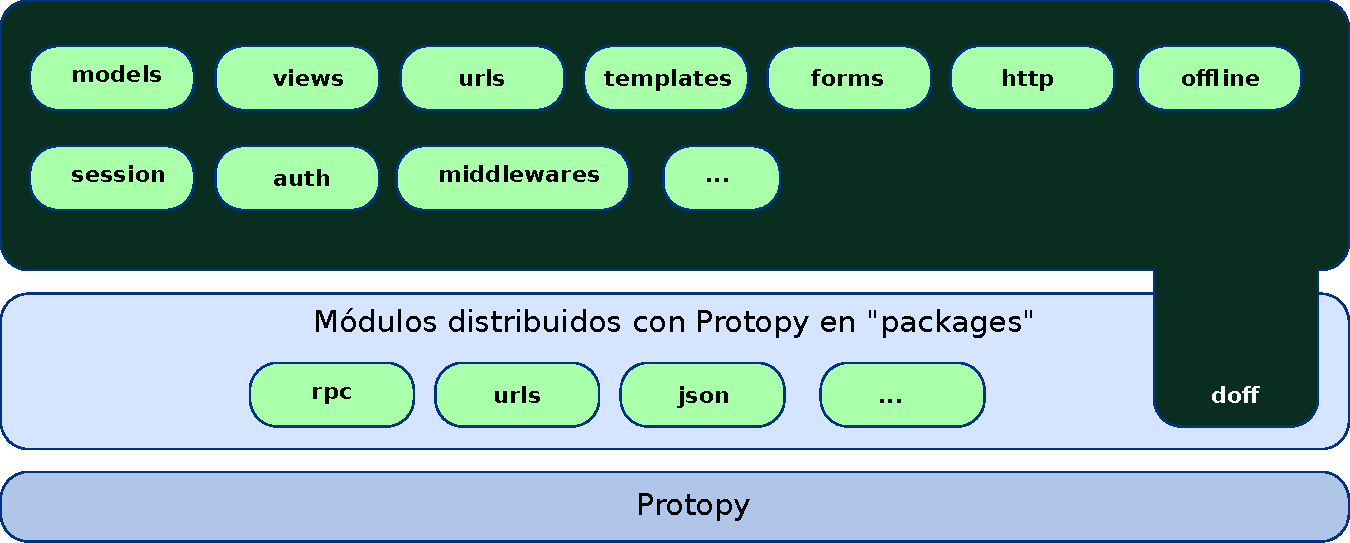
\includegraphics[scale=0.5]{esquema_doff.pdf}
}
\frame{
    \frametitle{Proyecto Desconectado}
    \begin{itemize}
        \item El desarrollador debe reescribir las vistas en JavaScript y URL en JavaScript.
        \item El desarrollador puede reutilizar los plantillas de Django
        \item El desarrollador {\bf debe reescribir} los modelos nuevamente JavaScript
    \end{itemize}
}

\frame{
    \frametitle{Offline - Objetivos}
    \itemize{        
        \item Automatización de creación de proyectos desconectados
        \item Servidor estático del código de Protopy y Doff
        \item Servidor estático del código de cada proyecto

    }
}

\frame{
    \frametitle{Offline - RemoteSites}
    \par{
        \par{\bf Objetivo}
        Definición de desconectado en el cliente. Cada sitio remoto es una {\it vista}
        de el proyecto y se publica en una {\it URL}

    }
    \itemize{
        
        \item Conversión de modelos de Python a JS mediante {\it introspección}
        
        \item Definición de acceso a datos del servidor
            \itemize{
                \item Acceso a filas ({\it managers})
                \item Acceso a columnas ({\it modificación de modelos})
            }
        \item Publicación de plantillas
        

        }


}

\frame{
    \frametitle{Offline - RemoteSites estructura}

    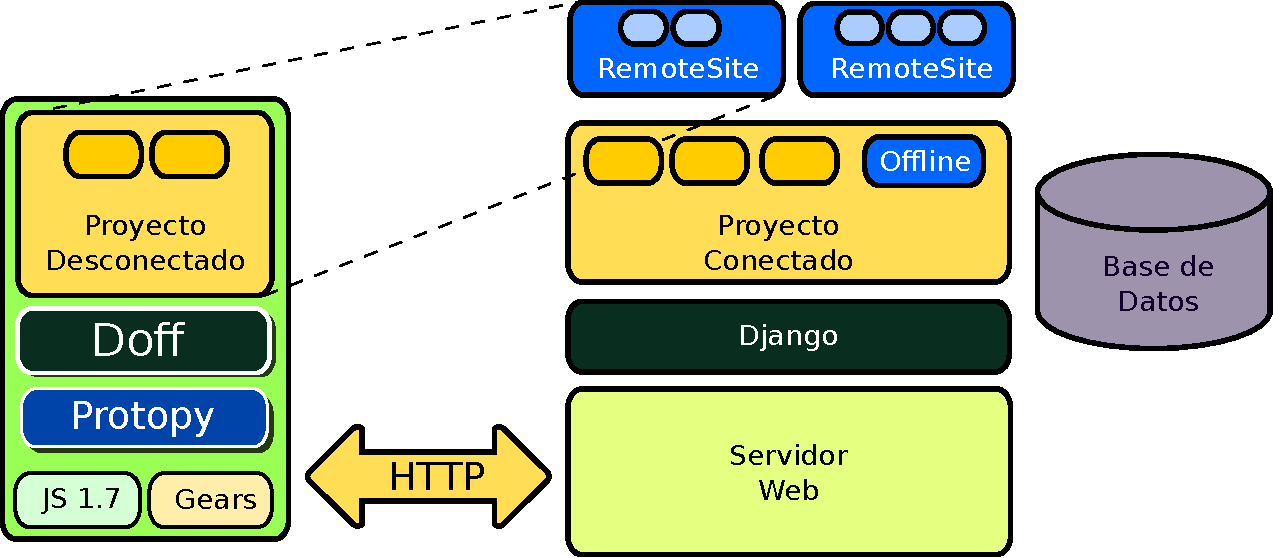
\includegraphics[scale=0.5]{remote_sites.pdf}
    
    
}

\section{Sincronización}
\frame{
    \frametitle{Esquema}
    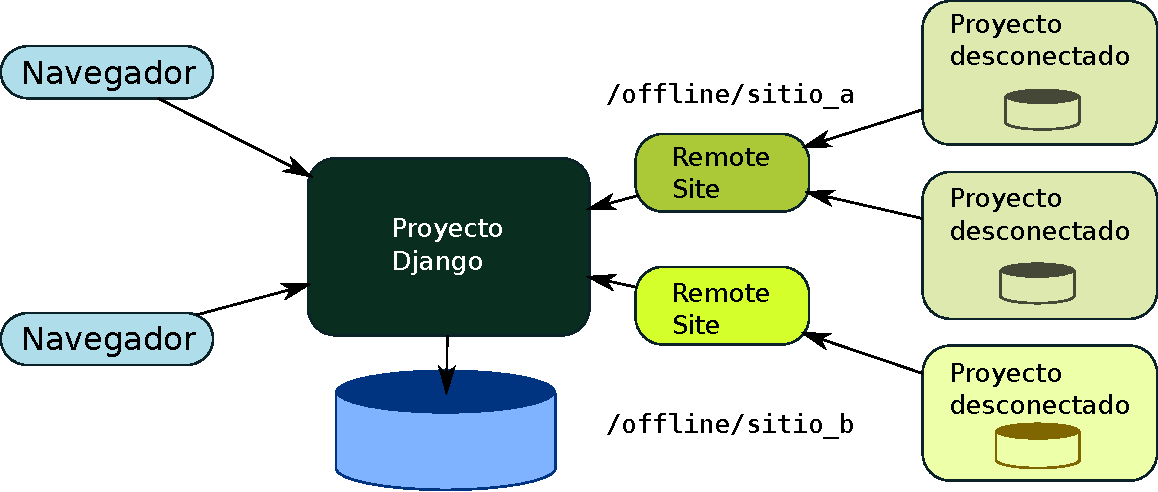
\includegraphics[scale=0.5]{esquema_distribuido.pdf}
}

\frame{
    \frametitle{Objetivo}
    \par {
    	Entidades definidas en el servidor se repliquen en el cliente y que las creadas y modificadas por el cliente
		se transfieran al servidor.
    }
    \begin{itemize}
        \item Integridad de la sincronización
		\item Transporte de datos
		\item Detección de cambios en instancias en el servidor
		\item Detección de cambios en el cliente
    \end{itemize}
}

\frame{
    \frametitle{Primitivas}
    \begin{itemize}
        \item {\bf PUSH}
        \item {\bf PULL}
        \item {\bf UPDATE}
        \item \textit{\bf PURGE}
    \end{itemize}
}

\frame{
    \frametitle{Conflictos}
    \begin{itemize}
        \item {\bf PUSH}
        \item {\bf PULL}
        \item {\bf UPDATE}
        \item \textit{\bf PURGE}
    \end{itemize}
}
\section{Conclusiones}
\frame{
    \frametitle{Conclusiones}
    \begin{itemize}
        \item {\bf Extender un framework}
        \item {\bf Persistencia del modelo de datos en el cliente}
        \item {\bf Acciones disponibles en modo desconectado}
        \item {\bf Primitivas de sincronización}
        \item {\bf Desarrollo de software libre} http://code.google.com/p/protopy
    \end{itemize}
}

\frame{
    \frametitle{Lineas Futuras}
    \begin{itemize}
        \item {\bf Conversión de Código Python en JavaScript}
        \item {\bf Sitio de Administración}
        \item {\bf Workers con Soporte para JavaScript 1.7}
        \item {\bf Compatibilidad con ES5 y HTML5}
        \item {\bf Optimizaciones en Base a Permanencia de Estado}
        \item {\bf Implementación de Storage o Almacenamiento en el Cliente}
        \item {\bf Compilación de JavaScript}
        \item {\bf Manejo de Migraciones de Esquema}
    \end{itemize}
}

\frame{
    \frametitle{Miscelánea}
    \begin{itemize}
        \item {\bf Firefox} Plataforma
        \item {\bf Firebug} Depuración
        \item {\bf Django} Framework Web
        \item {\bf Python} Lenguaje Server Side, Scripting, Sphinx Hacking, etc
        \item {\bf Mercurial} Control de versiones
        \item {\bf Sphinx} Para crear la documentación, \LaTeX{} y HTML
        \item {\bf \LaTeX{} - beamer} Para crear {\it esta} presentación
    \end{itemize}
}

\end{document}
